% !TeX root = ../main.tex
% Add the above to each chapter to make compiling the PDF easier in some editors.

\chapter{Introduction}
Modern sensors, sensor networks, computing systems and data-driven techniques have revolutionized the industry. As a key role in modern production facilities, prognostics and health management (PHM) applications have accelerated the big data revolution \cite{ZHAO2019213}. By analyzing production and machine data, the degradation status and risk of failure can be predicted for machines. This is especially helpful to increase the production quality and to reduce the downtime in production facilities \cite{Denkena2021}. Ball screw feed drives (BSDs) are common in industrial machines since they transfer rotary motion to linear motion with high precision \cite{LiPin2018}. Generally, BSDs are highly relevant for the entire machine’s precision, making its health condition monitoring especially interesting \cite{LiPin2018}. Surveys showed that BSDs are related in up to 19\% of all machine tool failures \cite{Denkena2021}. However, the research about modern health condition monitoring of BSDs is still in its early stages \cite{LiPin2018}. This thesis evaluates modern PHM systems to predict the degradation of BSDs.


\section{Relevance and Problems of Prognostics and Modern Health Management for Ball Screw Feed Drives}
BSDs represent an essential part of various industrial machines. Like all mechanical components that involve friction, BSDs also wear off. Especially the steel balls and screw shaft are significantly affected by degradation \cite{Pandhare2021}. In order to guarantee high motion repeatability while maximizing the expected life, the preload level of BSDs is calibrated precisely \cite{Pandhare2021}. The degradation of the BSD's components lowers the preload and therefore reduces the stiffness in the BSD system. This deteriorates the positioning accuracy and leads to a lower production quality or even a total machine failure \cite{Pandhare2021}. For this reason, health condition monitoring of BSDs is of great interest for the industry \cite{Pandhare2021}. The complex motion trajectory of the balls in BSDs and the difficult installation of sensors make the health condition monitoring of BSDs challenging \cite{LiPin2018}.

Due to the increasing computational power and amount of data, deep learning is considered a powerful and efficient method for extracting information from large datasets. Therefore, deep learning models have the ability to learn the mapping between machine data and machine health condition classes \cite{ZHAO2019213}. Unfortunately, many developed PHM models assume the training and testing dataset to have the same data distribution \cite{AZAMFAR2020103932}. In reality, this is not the case. If machines operate over long periods of time, their operational conditions change. This leads to changing fault characteristics in the machine data. Consequently, when applying PHM systems in real industrial scenarios over long periods of time, the systems' performance becomes unsatisfactory \cite{AZAMFAR2020103932}. The created domain shift between the training and testing data can be compensated by domain adaptation and transfer learning approaches, which measure and reduce the domain discrepancy between the two datasets while learning to solve the classification task \cite{AZAMFAR2020103932}.


\section{Traditional and Deep Learning Based Prognostics and Health Management Approaches}
As shown in figure \ref{fig:hand_crafted_features_physical_models_deep_learning}, PHM systems are traditionally restricted to physical-based and conventional data-driven approaches. Nowadays, deep learning has become more popular for extracting health condition information from machine data. Physical-based models explain the underlying complexity and degradation of machines with physical laws \cite{ZHAO2019213}. These models are especially advantageous since they do not require any historical fault data to make predictions \cite{Benker2019}. If the physics projected on the data does not consider all relevant machine aspects, including noise and perturbation, then the performance of such approaches is reduced \cite{ZHAO2019213}. In conventional data-driven approaches, traditional hand-crafted features are extracted from the machine data to retrieve expressive information about the machine's health condition. The features are rated by their suitability for the PHM task and the most promising ones are selected. Subsequently, a shallow classifier predicts the corresponding health condition of the machine \cite{ZHAO2019213}. The physical-based and conventional data-driven approaches suffer from several problems. Firstly, in complex real-world scenarios, establishing physical-based models or conventional hand-crafted features is a laborious task and requires much experience \cite{ZHAO2019213}. Secondly, an online model update is difficult \cite{ZHAO2019213}. Thirdly, the physical-based and conventional data-driven approaches are restricted to the specifications made about the monitoring task beforehand \cite{ZHAO2019213}. The limited transferability, flexibility and adaptability of these more traditional approaches are the reason for the growing interest in deep learning based PHM. Deep neural networks can capture relations within complex and high-dimensional data. Automatic learning makes neural networks easily adjustable to various problems \cite{ZHAO2019213}.
\begin{sidewaysfigure}
  \centering
  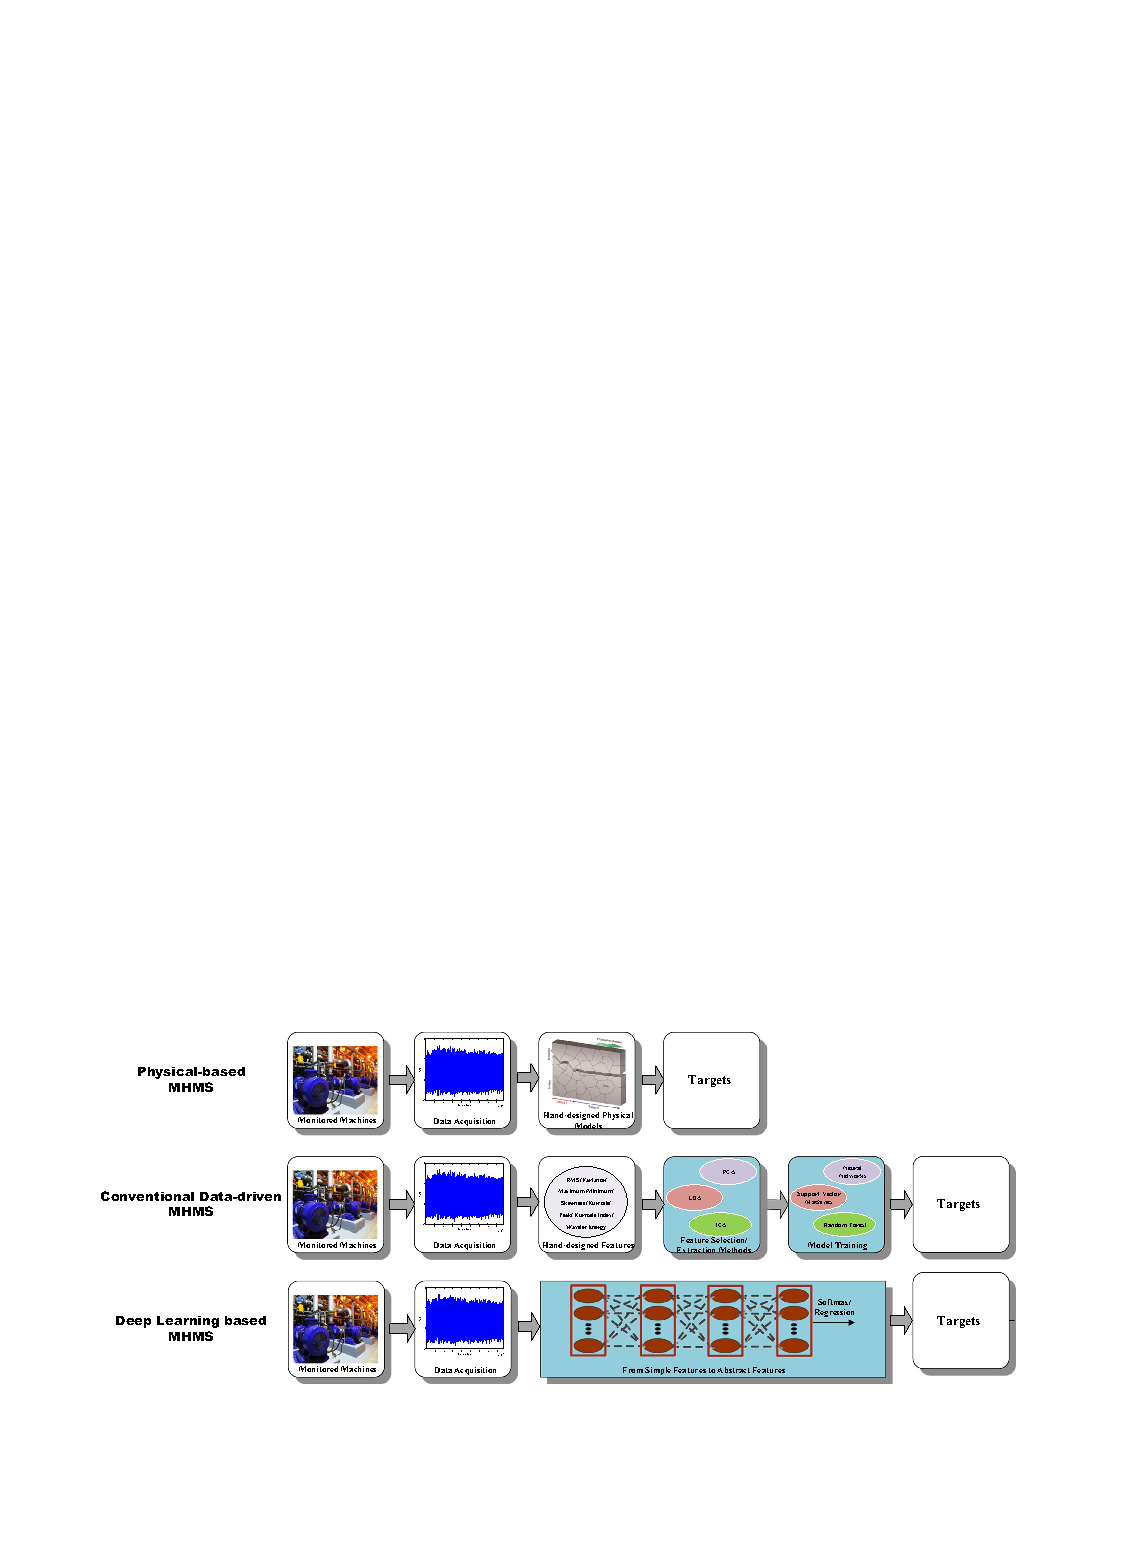
\includegraphics[width=1\textwidth]{hand_crafted_features_physical_models_deep_learning.pdf}
  \caption {Overview over traditional and deep learning based PHM approaches \cite{ZHAO2019213}} \label{fig:hand_crafted_features_physical_models_deep_learning}
\end{sidewaysfigure}
